% Options for packages loaded elsewhere
% Options for packages loaded elsewhere
\PassOptionsToPackage{unicode}{hyperref}
\PassOptionsToPackage{hyphens}{url}
\PassOptionsToPackage{dvipsnames,svgnames,x11names}{xcolor}
% Code above from https://github.com/quarto-dev/quarto-cli/blob/main/src/resources/formats/pdf/pandoc/passoptions.latex
% Customization below
\PassOptionsToPackage{babel}{csquotes}
%
\documentclass[
  french,
  11pt,
]{stylisharticle}
\usepackage{xcolor}
\usepackage{amsmath,amssymb}
\setcounter{secnumdepth}{2}
\usepackage{iftex}
\ifPDFTeX
  \usepackage[T1]{fontenc}
  \usepackage[utf8]{inputenc}
  \usepackage{textcomp} % provide euro and other symbols
\else % if luatex or xetex
  \usepackage{unicode-math} % this also loads fontspec
  \defaultfontfeatures{Scale=MatchLowercase}
  \defaultfontfeatures[\rmfamily]{Ligatures=TeX,Scale=1}
\fi
\usepackage{lmodern}
\ifPDFTeX\else
  % xetex/luatex font selection
\fi
% Use upquote if available, for straight quotes in verbatim environments
\IfFileExists{upquote.sty}{\usepackage{upquote}}{}
\IfFileExists{microtype.sty}{% use microtype if available
  \usepackage[]{microtype}
  \UseMicrotypeSet[protrusion]{basicmath} % disable protrusion for tt fonts
}{}
\makeatletter
\@ifundefined{KOMAClassName}{% if non-KOMA class
  \IfFileExists{parskip.sty}{%
    \usepackage{parskip}
  }{% else
    \setlength{\parindent}{0pt}
    \setlength{\parskip}{6pt plus 2pt minus 1pt}}
}{% if KOMA class
  \KOMAoptions{parskip=half}}
\makeatother
% Make \paragraph and \subparagraph free-standing
\makeatletter
\ifx\paragraph\undefined\else
  \let\oldparagraph\paragraph
  \renewcommand{\paragraph}{
    \@ifstar
      \xxxParagraphStar
      \xxxParagraphNoStar
  }
  \newcommand{\xxxParagraphStar}[1]{\oldparagraph*{#1}\mbox{}}
  \newcommand{\xxxParagraphNoStar}[1]{\oldparagraph{#1}\mbox{}}
\fi
\ifx\subparagraph\undefined\else
  \let\oldsubparagraph\subparagraph
  \renewcommand{\subparagraph}{
    \@ifstar
      \xxxSubParagraphStar
      \xxxSubParagraphNoStar
  }
  \newcommand{\xxxSubParagraphStar}[1]{\oldsubparagraph*{#1}\mbox{}}
  \newcommand{\xxxSubParagraphNoStar}[1]{\oldsubparagraph{#1}\mbox{}}
\fi
\makeatother


\usepackage{longtable,booktabs,array}
\newcounter{none} % for unnumbered tables
\usepackage{calc} % for calculating minipage widths
% Correct order of tables after \paragraph or \subparagraph
\usepackage{etoolbox}
\makeatletter
\patchcmd\longtable{\par}{\if@noskipsec\mbox{}\fi\par}{}{}
\makeatother
% Allow footnotes in longtable head/foot
\IfFileExists{footnotehyper.sty}{\usepackage{footnotehyper}}{\usepackage{footnote}}
\makesavenoteenv{longtable}
\usepackage{graphicx}
\makeatletter
\newsavebox\pandoc@box
\newcommand*\pandocbounded[1]{% scales image to fit in text height/width
  \sbox\pandoc@box{#1}%
  \Gscale@div\@tempa{\textheight}{\dimexpr\ht\pandoc@box+\dp\pandoc@box\relax}%
  \Gscale@div\@tempb{\linewidth}{\wd\pandoc@box}%
  \ifdim\@tempb\p@<\@tempa\p@\let\@tempa\@tempb\fi% select the smaller of both
  \ifdim\@tempa\p@<\p@\scalebox{\@tempa}{\usebox\pandoc@box}%
  \else\usebox{\pandoc@box}%
  \fi%
}
% Set default figure placement to htbp
\def\fps@figure{htbp}
\makeatother


% definitions for citeproc citations
\NewDocumentCommand\citeproctext{}{}
\NewDocumentCommand\citeproc{mm}{%
  \begingroup\def\citeproctext{#2}\cite{#1}\endgroup}
\makeatletter
 % allow citations to break across lines
 \let\@cite@ofmt\@firstofone
 % avoid brackets around text for \cite:
 \def\@biblabel#1{}
 \def\@cite#1#2{{#1\if@tempswa , #2\fi}}
\makeatother
\newlength{\cslhangindent}
\setlength{\cslhangindent}{1.5em}
\newlength{\csllabelwidth}
\setlength{\csllabelwidth}{3em}
\newenvironment{CSLReferences}[2] % #1 hanging-indent, #2 entry-spacing
 {\begin{list}{}{%
  \setlength{\itemindent}{0pt}
  \setlength{\leftmargin}{0pt}
  \setlength{\parsep}{0pt}
  % turn on hanging indent if param 1 is 1
  \ifodd #1
   \setlength{\leftmargin}{\cslhangindent}
   \setlength{\itemindent}{-1\cslhangindent}
  \fi
  % set entry spacing
  \setlength{\itemsep}{#2\baselineskip}}}
 {\end{list}}
\usepackage{calc}
\newcommand{\CSLBlock}[1]{\hfill\break\parbox[t]{\linewidth}{\strut\ignorespaces#1\strut}}
\newcommand{\CSLLeftMargin}[1]{\parbox[t]{\csllabelwidth}{\strut#1\strut}}
\newcommand{\CSLRightInline}[1]{\parbox[t]{\linewidth - \csllabelwidth}{\strut#1\strut}}
\newcommand{\CSLIndent}[1]{\hspace{\cslhangindent}#1}

\ifLuaTeX
\usepackage[bidi=basic,shorthands=off]{babel}
\else
\usepackage[bidi=default,shorthands=off]{babel}
\fi
\ifLuaTeX
  \usepackage{selnolig} % disable illegal ligatures
\fi


\setlength{\emergencystretch}{3em} % prevent overfull lines

\providecommand{\tightlist}{%
  \setlength{\itemsep}{0pt}\setlength{\parskip}{0pt}}



 

\usepackage[]{csquotes}

% -------------- Additional packages
\usepackage{orcidlink}  % Orcid logo and link to author page

% -------------- Font size
% R output: footnotesize
\makeatletter
\patchcmd{\@verbatim}
  {\verbatim@font}
  {\verbatim@font\footnotesize}
  {}{}
% References font size whether bibtex is used or not
\@ifundefined{bibfont}
  {%
    \AtBeginEnvironment{CSLReferences}{\footnotesize}
  }
  {%
    \renewcommand*{\bibfont}{\footnotesize}
  }%
\makeatother

% -------------- longtable 2 columns
% https://tex.stackexchange.com/questions/161431/how-to-solve-longtable-is-not-in-1-column-mode-error
\makeatletter
\let\oldlt\longtable
\let\endoldlt\endlongtable
\def\longtable{\@ifnextchar[\longtable@i \longtable@ii}
\def\longtable@i[#1]{
\begin{figure}[t]
\onecolumn
\begin{minipage}{0.5\textwidth}\scriptsize
\oldlt[#1]
}
\def\longtable@ii{
\begin{figure}[t]
\onecolumn
\begin{minipage}{0.5\textwidth}\scriptsize
\oldlt
}
\definecolor{red}{RGB}{255, 0, 0}
\definecolor{green}{RGB}{0, 255, 0}
\definecolor{blue}{RGB}{0, 0, 255}
\definecolor{grey}{RGB}{191, 191, 191}
\makeatletter
\@ifpackageloaded{caption}{}{\usepackage{caption}}
\AtBeginDocument{%
\ifdefined\contentsname
  \renewcommand*\contentsname{Table des matières}
\else
  \newcommand\contentsname{Table des matières}
\fi
\ifdefined\listfigurename
  \renewcommand*\listfigurename{Liste des Figures}
\else
  \newcommand\listfigurename{Liste des Figures}
\fi
\ifdefined\listtablename
  \renewcommand*\listtablename{Liste des Tables}
\else
  \newcommand\listtablename{Liste des Tables}
\fi
\ifdefined\figurename
  \renewcommand*\figurename{Figure}
\else
  \newcommand\figurename{Figure}
\fi
\ifdefined\tablename
  \renewcommand*\tablename{Table}
\else
  \newcommand\tablename{Table}
\fi
}
\@ifpackageloaded{float}{}{\usepackage{float}}
\floatstyle{ruled}
\@ifundefined{c@chapter}{\newfloat{codelisting}{h}{lop}}{\newfloat{codelisting}{h}{lop}[chapter]}
\floatname{codelisting}{Listing}
\newcommand*\listoflistings{\listof{codelisting}{Liste des Listings}}
\makeatother
\makeatletter
\makeatother
\makeatletter
\@ifpackageloaded{caption}{}{\usepackage{caption}}
\@ifpackageloaded{subcaption}{}{\usepackage{subcaption}}
\makeatother
\usepackage{bookmark}
\IfFileExists{xurl.sty}{\usepackage{xurl}}{} % add URL line breaks if available
\urlstyle{same}
\hypersetup{
  pdftitle={Étude comparative de la diversité des forêts de Paracou et de BCI},
  pdfauthor={Martin Boucknooghe},
  pdflang={fr-FR},
  pdfkeywords={template, demo},
  colorlinks=true,
  linkcolor={blue},
  filecolor={Maroon},
  citecolor={Blue},
  urlcolor={blue},
  pdfcreator={LaTeX via pandoc}}


% Set up hyperref, after loading it
\hypersetup{
  linkcolor=black,
  citecolor=black,
  colorlinks=true
}

% Journal information
  \JournalInfo{Publication reference}

% Additional notes (e.g. copyright, DOI, review/research article)
  \Archive{DOI: xxx/xx}

% Article title
\PaperTitle{Étude comparative de la diversité des forêts de Paracou et
de BCI}

% Authors
\Authors{
      {Martin Boucknooghe}%
    \textsuperscript{%
      ~\orcidlink{0000-0000-0000-0000}%
      1%
      %
    }%
    }

% Affiliations
    \affiliation{%
      \textsuperscript{1}%
      Université de Montpellier%
      , Département Scientifique%
      %
      , Somewhere%
      , Montpellier%
      %
      , France%
      , 34000%
      %
    }

% Corresponding author
  %

% Keywords
\Keywords{template, demo}
\newcommand{\keywordname}{Keywords} % Defines the keywords heading name

%	Abstract
\Abstract{
  Cette étude compare la diversité de deux forêts tropicales
  intensivement étudiées, Paracou (Guyane française) et Barro Colorado
  Island (Panama).
}
\begin{document}
% Makes all text pages the same height
\flushbottom

% Print the title and abstract box
\maketitle

% Print the contents section
\tableofcontents

% Remove page numbering from the first page
\thispagestyle{empty}

\section{Introduction}\label{introduction}

\begin{itemize}
\tightlist
\item
  La diversité des forêts tropicales fascine les écologues en raison de
  ses enjeux majeurs ({Gibson et al.} 2011).
\item
  Des modèles récents proposent des explications fondées sur la
  dynamique démographique ({Liang et al.} 2022).
\item
  Dans un contexte de menaces croissantes sur la biodiversité ({Fadrique
  et al.} 2026), nous comparons ici deux forêts tropicales intensivement
  étudiées, Paracou et BCI, afin de déterminer si des sites aux
  conditions contrastées présentent des patrons de diversité
  comparables.
\end{itemize}

\section{Matériels et méthodes}\label{matuxe9riels-et-muxe9thodes}

Présentation du site de Paracou.

\begin{itemize}
\tightlist
\item
  Localisation : Le site se trouve à environ 50 kilomètres de Kourou.
\item
  Superficie : Il s'étend sur 500 hectares de forêt tropicale humide
  très riche en biodiversité.
\item
  Création : Le CIRAD a mis en place ce dispositif de recherche en 1982
\item
  Objectifs scientifiques

  \begin{itemize}
  \item
    Étude de la forêt : Les scientifiques observent le fonctionnement de
    la forêt tropicale et sa dynamique.
  \item
    Impact des perturbations : Le site teste des niveaux d'intervention
    humaine, comme l'exploitation forestière.
  \item
    Climat et carbone : Les chercheurs mesurent les échanges de gaz
    carbonique entre la forêt et l'atmosphère.
  \end{itemize}
\end{itemize}

\begin{itemize}
\tightlist
\item
  Présentation du site de BCI.
\end{itemize}

\begin{itemize}
\tightlist
\item
  Valeur de la diversité en fonction de son ordre (Tothmeresz 1995;
  Patil et Taillie 1982).
\end{itemize}

\section{Résultats}\label{ruxe9sultats}

\begin{itemize}
\tightlist
\item
  Diversité Comparative
\end{itemize}

\begin{figure}

\centering{

\pandocbounded{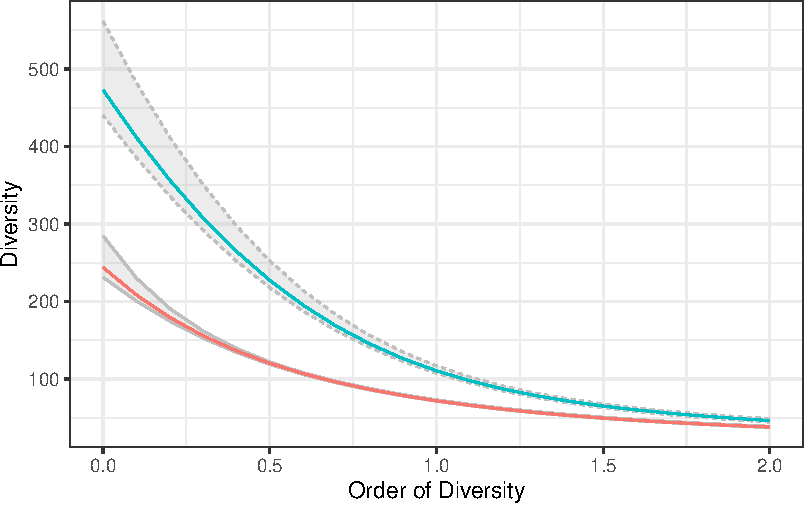
\includegraphics[keepaspectratio]{index_files/figure-pdf/unnamed-chunk-1-1.pdf}}

}

\caption{\label{fig-diversite_comparaison}Profils de diversité de
Paracou parcelle 6 (courbe bleue) et BCI (courbe rouge). La figure
représente le nombre effectif d'espèces (nombre de Hill) en fonction de
l'ordre de la diversité.}

\end{figure}%

\section{Discussion}\label{discussion}

\begin{itemize}
\item
  Cette étude met en évidence à la fois des similitudes et des
  différences entre la diversité de Paracou et BCI.
\item
  Similitudes : les deux sites présentent une forte richesse spécifique.
\item
  Différences : les abondances relatives et la composition changent.
\item
  Les écarts observés s'explique par des différences biogéographique, de
  perturbation, de sols ou d'histoire .
\item
  MacArthur et Wilson (1967) montrent mathématiquement que la richesse
  spécifique (le nombre d'espèces) d'une île est un équilibre dynamique
  entre le taux d'immigration et le taux d'extinction, ce dernier étant
  directement dicté par la taille de l'île.
\item
  BCI est une forêt secondarisée (Raby 2017). Sa diversité pourrait être
  augmentée selon la théorie de la perturbation intermédiaire (Connell
  1978).
\end{itemize}

\section*{References}\label{bibliography}
\addcontentsline{toc}{section}{References}

\protect\phantomsection\label{refs}
\begin{CSLReferences}{1}{1}
\bibitem[\citeproctext]{ref-Connell1978}
Connell, Joseph H. 1978. {«~Diversity in tropical rain forests and coral
reefs~»}. \emph{Science} 199 (4335): 1302‑10.
\url{https://doi.org/10.1126/science.199.4335.1302}.

\bibitem[\citeproctext]{ref-Fadrique2026}
{Fadrique, B., F. Costa, F. Cuesta, et al.} 2026. {«~Tree diversity is
changing across tropical Andean and Amazonian forests in response to
global change~»}. \emph{Nature Ecology \& Evolution} 10 (2): 267‑80.
\url{https://doi.org/10.1038/s41559-025-02956-5}.

\bibitem[\citeproctext]{ref-Gibson2011}
{Gibson, Luke, Tien Ming Lee, Lian Pin Koh, et al.} 2011. {«~Primary
forests are irreplaceable for sustaining tropical biodiversity~»}.
\emph{Nature} 478 (7369): 378‑81.
\url{https://doi.org/10.1038/nature10425}.

\bibitem[\citeproctext]{ref-Liang2022}
{Liang, Jingjing, Javier G. P. Gamarra, Nicolas Picard, et al.} 2022.
{«~Co-limitation towards lower latitudes shapes global forest diversity
gradients~»}. \emph{Nature Ecology \& Evolution} 6 (août): 1423‑37.
\url{https://doi.org/10.1038/s41559-022-01831-x}.

\bibitem[\citeproctext]{ref-MacArthur1967}
MacArthur, Robert H., et Edward O. Wilson. 1967. \emph{The theory of
island biogeography}. Monographs in population biology. Princeton
University Press.

\bibitem[\citeproctext]{ref-Patil1982}
Patil, Ganapati P., et Charles Taillie. 1982. {«~Diversity as a concept
and its measurement~»}. \emph{Journal of the American Statistical
Association} 77 (379): 548‑61. \url{https://doi.org/10.2307/2287709}.

\bibitem[\citeproctext]{ref-Raby2017}
Raby, Megan. 2017. \emph{American tropics: the Caribbean roots of
biodiversity science}. Flows, migrations, et exchanges. The University
of North Carolina Press.

\bibitem[\citeproctext]{ref-Tothmeresz1995}
Tothmeresz, Béla. 1995. {«~Comparison of different methods for diversity
ordering~»}. \emph{Journal of Vegetation Science} 6 (2): 283‑90.
\url{https://doi.org/10.2307/3236223}.

\end{CSLReferences}




\end{document}
